
% \section{Introduzione al capitolo}\label{sec:intro_cap3}


% Avendo chiarito il fondamento scientifico e tecnologico nel \cref{chap:contesto}, presentiamo ora il prototipo di LLM Query Builder realizzato come soluzione concreta ai problemi identificati.

% Questo capitolo è organizzato secondo una prospettiva \textit{user-centered}: partiamo dal dominio di applicazione (DH.ARC e il Datavault) e dal profilo degli utenti target (\cref{sec:dominio}), passiamo all'architettura funzionale del sistema come appare all'utente (\cref{sec:architettura}), e concludiamo con tre scenari d'uso concreti (\cref{sec:casiduso}) che dimostrano il valore aggiunto della nostra proposta.


% \section{Il dominio e gli utenti target}\label{sec:dominio}


% \subsection{Il contesto operativo: DH.ARC e il Datavault}\label{subsec:dharc}

% Il Digital Humanities Advanced Research Centre (DH.ARC) è un polo di ricerca dell'Università di Bologna afferente al Dipartimento di Filologia Classica e Italianistica (FICLIT), nato con l'obiettivo di ``connettere studenti, ricercatori, personale IT e professori del FICLIT e del Dipartimento di Informatica --- Scienza e Ingegneria (DISI)''\cite{Ams26}.

% Il centro ha lo scopo di fungere da hub per gli studiosi e le istituzioni, supportandoli ``nella progettazione, sviluppo e manutenzione di progetti di ricerca DH'' e promuovendo iniziative innovative nel campo umanistico.

% Le attività di ricerca vertono prevalentemente sulla digitalizzazione e creazione di metadati per il patrimonio culturale, che includono in gran parte ``documenti archivistici e libri antichi'', ``testi letterari'' e ``knowledge graphs che descrivono oggetti del patrimonio culturale'' come fotografie e opere d'arte.

% In questo ecosistema si inserisce il \textit{Datavault}, un database RDF (basato su Blazegraph) che funge da enorme bacino di immagazzinamento delle informazioni. Il Datavault ``contiene, ad ora, 19 milioni di triple tutte molto simili'', dotate di uno specifico ``schema RDF reale''. Proprio a causa di questa vastità e similarità strutturale, ``andare a cercare il file specifico non è cosa semplice ed immediata'': attualmente manca infatti un modo per ``interrogare i dati per contenuto o concetto, nonostante Blazegraph renda l'informazione potenzialmente ricercabile in modo flessibile''.

% \subsection{Profilo dell'utente finale: i ricercatori del centro}\label{subsec:utenti}

% \subsubsection{Profilo disciplinare e competenze tecniche}

% L'utenza di riferimento del centro DH.ARC è composta da docenti, ricercatori, assegnisti e studenti di discipline prettamente umanistiche, quali filologia, storia, storia dell'arte e archeologia\cite{Per22}. Questi studiosi sono molto competenti nel dominio delle fonti culturali e nell'analisi dei testi critici, ma tipicamente sono privi di un background informatico formale. 

% La loro alfabetizzazione digitale nel campo dell'Information Retrieval si limita solitamente all'impiego di strumenti ``pronti all'uso'': cataloghi OPAC, database relazionali con maschere pre-configurate o motori di ricerca generici. Non hanno familiarità con triplestore RDF, SPARQL, o Knowledge Graphs.

% \subsubsection{Caratterizzazione dei bisogni informativi}

% In questo ecosistema, gli utenti non ricercano identificativi esatti o risposte chiuse; piuttosto, adottano comportamenti di ricerca esplorativa, procedendo per esplorazione libera al fine di collegare concetti e scoprire associazioni non immediate tra i documenti.

% Interrogando il Datavault, gli umanisti del centro necessitano di porre interrogazioni cross-dominio articolate, formulando mentalmente domande come: 
% \begin{quote}
% ``Quali immagini di codici medievali del XIV secolo sono state digitalizzate con risoluzione superiore a 300 dpi nel corso del progetto X?\@''
% \end{quote}
% o ancora:
% \begin{quote}
% ``Mostrami tutti i manoscritti attribuiti a un determinato autore e digitalizzati nell'ultimo anno''.
% \end{quote}


% \section{Architettura Funzionale (Ad alto livello)}\label{sec:architettura}


% \subsection{Il flusso dell'interazione}\label{subsec:flusso}

% Dal punto di vista dell'utente, il sistema funziona secondo un flusso semplice:

% \begin{enumerate}
%     \item \textbf{Input}: l'utente apre l'interfaccia del Datavault Browser, trova una barra di ricerca testuale (LLM Search Bar), e digita la sua domanda in italiano in forma libera. Non ci sono campi da compilare, sintassi da rispettare, o vocabolari controllati da imparare.
    
%     Esempio: ``Mostrami tutte le immagini scansionate con una fotocamera Nikon nel 2022''.
    
%     \item \textbf{Elaborazione}: il testo naturale viene inviato a un componente intelligente (il modello LLM fine-tuned) che, guidato dalla conoscenza dell'ontologia del Datavault, produce una query SPARQL corrispondente.
    
%     \item \textbf{Output}: la query SPARQL viene eseguita sul Datavault (Blazegraph) e i risultati vengono restituiti e visualizzati nell'interfaccia come un albero di risorse navigabile. L'utente non vede mai la query SPARQL a meno che non la voglia; vede solo i risultati pertinenti alla sua domanda.
% \end{enumerate}

% \subsection{Diagramma funzionale del sistema}\label{subsec:diagramma}

% % TODO: Inserire un diagramma TikZ o un'immagine che illustri il flusso
% % [Input testuale] -> [LLM Query Builder] -> [SPARQL Query] -> [Blazegraph] -> [Risultati]
% %
% % Per ora lasciare uno spazio riservato con \cref{fig:diagramma_funzionale}

% \subsection{I componenti del sistema e le loro responsabilità}\label{subsec:componenti}

% Il sistema si articola in tre componenti principali:

% \begin{enumerate}
%     \item \textbf{Frontend (Datavault Browser)}: interfaccia utente dove l'utente digita le domande e visualizza i risultati. Responsabile di: raccogliere input testuale, inviarlo al backend, visualizzare i risultati in formato navigabile.
    
%     \item \textbf{Backend (LLM Query Builder + RAG Engine)}: il ``cervello'' del sistema. Responsabile di: ricevere la domanda naturale, recuperare lo schema RDF e predicati rilevanti dal Datavault, generare una query SPARQL utilizzando il modello LLM fine-tuned, gestire errori e allucinazioni.
    
%     \item \textbf{Data Layer (Blazegraph + Schema RDF)}: il triplestore vero e proprio. Responsabile di: immagazzinare e gestire i 19 milioni di triple RDF, eseguire la query SPARQL generata dal backend, restituire i risultati al componente precedente.
% \end{enumerate}


% \section{Casi d'uso principali}\label{sec:casiduso}


% Descriviamo tre scenari d'uso concreti che rappresentano i bisogni tipici della ricerca presso DH.ARC:\@

% \subsection{Caso d'uso 1: ricerca per caratteristiche di acquisizione}\label{subsec:cu1}

% \textbf{Attore}: un ricercatore che vuole individuare immagini acquisite con specifiche caratteristiche tecniche.

% \textbf{Obiettivo}: trovare tutte le immagini di una collezione digitalizzate con uno specifico dispositivo fotografico e in un dato intervallo temporale.

% \textbf{Input}: ``Mostrami tutte le immagini scansionate con una Nikon D850 tra il 2021 e il 2023''.

% \textbf{Traducibilità manuale in SPARQL}: sarebbe complesso e richiederebbe conoscenza di \code{exif:make}, \code{exif:dateTime}, e gestione di range temporali.

% \textbf{Rilevanza}: Questo caso d'uso dimostra come il sistema gestisce filtri tecnici (dispositivo fotografico) combinati con vincoli temporali, delegando all'LLM la complessità di tradurre una descrizione naturale in una query strutturata.

% \subsection{Caso d'uso 2: ricerca per progetto e tipologia di risorsa}\label{subsec:cu2}

% \textbf{Attore}: un responsabile di un progetto di digitalizzazione che vuole fare un inventario delle risorse prodotte.

% \textbf{Obiettivo}: elencare tutte le risorse di un progetto specifico con una determinata tipologia.

% \textbf{Input}: ``Elenca tutte le risorse del progetto NextScan caricate nel sistema''.

% \textbf{Traducibilità manuale in SPARQL}: richiede conoscenza di predicati descrittivi (\code{dc:isPartOf}, \code{dc:title}) e della struttura dei progetti nel Datavault.

% \textbf{Rilevanza}: Questo caso d'uso dimostra la capacità del sistema di filtrare per metadati descrittivi (Dublin Core) anziché tecnici (EXIF), rispondendo a un bisogno amministrativo frequente nel dominio DH.ARC.\@

% \subsection{Caso d'uso 3: ricerca multi-criterio con filtro temporale}\label{subsec:cu3}

% \textbf{Attore}: un ricercatore che vuole analizzare la produzione digitale in un periodo specifico.

% \textbf{Obiettivo}: trovare tutte le risorse acquisite in un intervallo temporale con ulteriori vincoli di qualità.

% \textbf{Input}: ``Mostrami tutte le risorse acquisite tra il 2022 e il 2023 con una risoluzione superiore a 4000 pixel''.

% \textbf{Traducibilità manuale in SPARQL}: è il caso più complesso---dimostra la capacità del sistema di gestire query multi-criterio (filtri combinati su data E caratteristica tecnica), estremamente difficili da scrivere manualmente in SPARQL per un non esperto.

% \textbf{Rilevanza}: Questo è il caso d'uso più forte per la nostra proposta: evidenzia il valore aggiunto del sistema rispetto ai filtri tradizionali e alla scrittura manuale di SPARQL.\@


% \section{Conclusioni del capitolo}\label{sec:conclusioni_cap3}
% In questo capitolo abbiamo presentato il prototipo di LLM Query Builder nel suo contesto operativo e funzionale. Abbiamo visto che:

% \begin{enumerate}
%     \item Il dominio di applicazione (DH.ARC) presenta utenti con bisogni esplorativi complessi e assenza di competenze tecniche;
%     \item L'architettura funzionale del sistema è semplice dal punto di vista dell'utente: ``domanda naturale $\to$ risultati'', nascondendo tutta la complessità nel backend;
%     \item I tre casi d'uso concreti dimostrano come il sistema riduce significativamente la barriera di accesso al Datavault.
% \end{enumerate}

% Avendo chiarito il \textit{cosa} e il \textit{perché}, il \cref{chap:implementazione} approfondisce le scelte architetturali e implementative che rendono possibile il funzionamento del sistema: la struttura del backend LLM, il processo di fine-tuning del modello, la gestione dell'ontologia RDF, e la progettazione del dataset di training.

\section{Introduzione al capitolo}\label{sec:intro_cap3}

Avendo chiarito il fondamento scientifico e tecnologico nel \cref{chap:contesto}, presentiamo ora il prototipo di LLM Query Builder realizzato come soluzione concreta ai problemi identificati.

Questo capitolo è organizzato secondo una prospettiva \textit{user-centered}: partiamo dal dominio di applicazione (DH.ARC e il Datavault) e dal profilo degli utenti target (\cref{sec:dominio}), passiamo all'architettura funzionale e all'interfaccia del sistema (\cref{sec:architettura}), e concludiamo con tre scenari d'uso concreti (\cref{sec:casiduso}) arricchiti dalle relative schermate, per dimostrare il valore aggiunto della nostra proposta.

\section{Il dominio e gli utenti target}\label{sec:dominio}

\subsection{Il contesto operativo: DH.ARC e il Datavault}\label{subsec:dharc}
Il Digital Humanities Advanced Research Centre (DH.ARC) è un polo di ricerca dell'Università di Bologna afferente al Dipartimento di Filologia Classica e Italianistica (FICLIT), nato con l'obiettivo di ``connettere studenti, ricercatori, personale IT e professori del FICLIT e del Dipartimento di Informatica --- Scienza e Ingegneria (DISI)''\hfill\cite{Ams26}.

Il centro ha lo scopo di fungere da hub per gli studiosi e le istituzioni, supportandoli ``nella progettazione, sviluppo e manutenzione di progetti di ricerca DH'' e promuovendo iniziative innovative nel campo umanistico.

Le attività di ricerca vertono prevalentemente sulla digitalizzazione e creazione di metadati per il patrimonio culturale, che includono in gran parte ``documenti archivistici e libri antichi'', ``testi letterari'' e ``knowledge graphs che descrivono oggetti del patrimonio culturale'' come fotografie e opere d'arte.

In questo ecosistema si inserisce il \textit{Datavault}, un database RDF (basato su Blazegraph) che funge da enorme bacino di immagazzinamento delle informazioni. Il Datavault ``contiene, ad ora, 19 milioni di triple tutte molto simili'', dotate di uno specifico ``schema RDF reale''. Proprio a causa di questa vastità e similarità strutturale, ``andare a cercare il file specifico non è cosa semplice ed immediata'': attualmente manca infatti un modo per ``interrogare i dati per contenuto o concetto, nonostante Blazegraph renda l'informazione potenzialmente ricercabile in modo flessibile''.

\subsection{Profilo dell'utente finale: i ricercatori del centro}\label{subsec:utenti}

\subsubsection{Profilo disciplinare e competenze tecniche}
L'utenza di riferimento del centro DH.ARC è composta da docenti, ricercatori, assegnisti e studenti di discipline prettamente umanistiche, quali filologia, storia, storia dell'arte e archeologia\cite{Per22}. Questi studiosi sono molto competenti nel dominio delle fonti culturali e nell'analisi dei testi critici, ma tipicamente sono privi di un background informatico formale. 

La loro alfabetizzazione digitale nel campo dell'Information Retrieval si limita solitamente all'impiego di strumenti ``pronti all'uso'': cataloghi OPAC, database relazionali con maschere pre-configurate o motori di ricerca generici. Non hanno familiarità con triplestore RDF, SPARQL, o Knowledge Graphs.

\subsubsection{Caratterizzazione dei bisogni informativi}
In questo ecosistema, gli utenti non ricercano identificativi esatti o risposte chiuse; piuttosto, adottano comportamenti di ricerca esplorativa, procedendo per esplorazione libera al fine di collegare concetti e scoprire associazioni non immediate tra i documenti.

Interrogando il Datavault, gli umanisti del centro necessitano di porre interrogazioni cross-dominio articolate, formulando mentalmente domande come: 
\begin{quote}
``Quali immagini di codici medievali del XIV secolo sono state digitalizzate con risoluzione superiore a 300 dpi nel corso del progetto X?\@''
\end{quote}
o ancora:
\begin{quote}
``Mostrami tutti i manoscritti attribuiti a un determinato autore e digitalizzati nell'ultimo anno''.
\end{quote}

\section{Architettura Funzionale e Interfaccia Utente}\label{sec:architettura}

\subsection{L'interfaccia: come si usa il Data Vault Explorer}\label{subsec:interfaccia}
Per risolvere i problemi di carico cognitivo e rigidità formale descritti nel capitolo precedente, il sistema si presenta all'utente attraverso un'interfaccia minimalista e conversazionale (il Data Vault Explorer). L'utente non si trova di fronte a form complessi o ontologie da studiare, ma a un singolo punto di ingresso: la LLM Search Bar.

\begin{figure}[H]
    \centering
    
\includegraphics[width=0.9\textwidth]{img/schermata_principale.png}
    \caption{L'interfaccia principale del Data Vault Explorer con la LLM Search Bar.}\label{fig:schermata_principale}
\end{figure}

Come visibile in \cref{fig:schermata_principale}, l'impiego del sistema si riduce a un'azione elementare: digitare il proprio bisogno informativo in italiano naturale. Il sistema restituisce i risultati strutturandoli in un albero di risorse navigabile, garantendo un'esplorazione fluida e intuitiva dei dati.

\subsection{Il flusso dell'interazione}\label{subsec:flusso}
Dal punto di vista dell'utente, il sistema funziona secondo un flusso invisibile ma rigoroso:

\begin{enumerate}
    \item \textbf{Input}: l'utente digita la domanda in italiano in forma libera. Non ci sono campi da compilare né sintassi da rispettare.
    \item \textbf{Elaborazione}: il testo naturale viene inviato a un componente intelligente (il modello LLM fine-tuned) che, guidato dalla conoscenza dell'ontologia del Datavault, produce autonomamente la query SPARQL corrispondente.
    \item \textbf{Output}: la query SPARQL viene eseguita su Blazegraph. L'utente non vede mai il codice (salvo esplicita richiesta), ma visualizza esclusivamente i risultati pertinenti, aggirando completamente la barriera del linguaggio formale.
\end{enumerate}

\subsection{I componenti del sistema e le loro responsabilità}\label{subsec:componenti}
Il sistema si articola in tre componenti principali:
\begin{enumerate}
    \item \textbf{Frontend (Data Vault Explorer)}: raccoglie l'input testuale e renderizza i risultati in formato navigabile.
    \item \textbf{Backend (LLM Query Builder + RAG Engine)}: il ``cervello'' del sistema. Riceve la domanda, recupera lo schema RDF, genera la query SPARQL tramite il modello e gestisce gli errori semantici (evitando le allucinazioni).
    \item \textbf{Data Layer (Blazegraph + Schema RDF)}: immagazzina i 19 milioni di triple ed esegue l'interrogazione generata dal backend.
\end{enumerate}

\section{Casi d'uso principali ed esempi}\label{sec:casiduso}

Descriviamo tre scenari d'uso concreti che dimostrano l'efficacia del sistema presso DH.ARC, evidenziando il parallelismo tra l'interazione logica (traduzione LLM e sanitizzazione) e il riscontro visivo restituito all'utente.\@

\subsection{Caso d'uso 1: ricerca per caratteristiche di acquisizione e gestione anomalie}\label{subsec:cu1}
\textbf{Attore}: un ricercatore che vuole individuare immagini acquisite con specifiche caratteristiche tecniche.\\
\textbf{Input testuale}: ``Filtra i risultati mostrandomi le risorse acquisite con il dispositivo NextScan''.

\begin{figure}[H]
    \centering
    \begin{minipage}[c]{0.48\textwidth}
\begin{lstlisting}[basicstyle=\ttfamily\scriptsize, breaklines=true]
PREFIX exif: <http://wwww3org/2003/12/exif/ns#>
PREFIX fedora: <http://fedora.info/definitions/v4/repository#>
PREFIX ebucore: <http://www.ebu.ch/metadata/ontologies/ebucore/ebucore#>
PREFIX ldp: <http://www.w3.org/ns/ldp#>
PREFIX dc: <http://purl.org/dc/elements/1.1/>

SELECT DISTINCT ?image WHERE {
  ?image exif:make ?make .
  FILTER(CONTAINS(LCASE(?make), "nextscan"))
}
LIMIT 20
\end{lstlisting}
    \end{minipage}\hfill
    \begin{minipage}[c]{0.48\textwidth}
        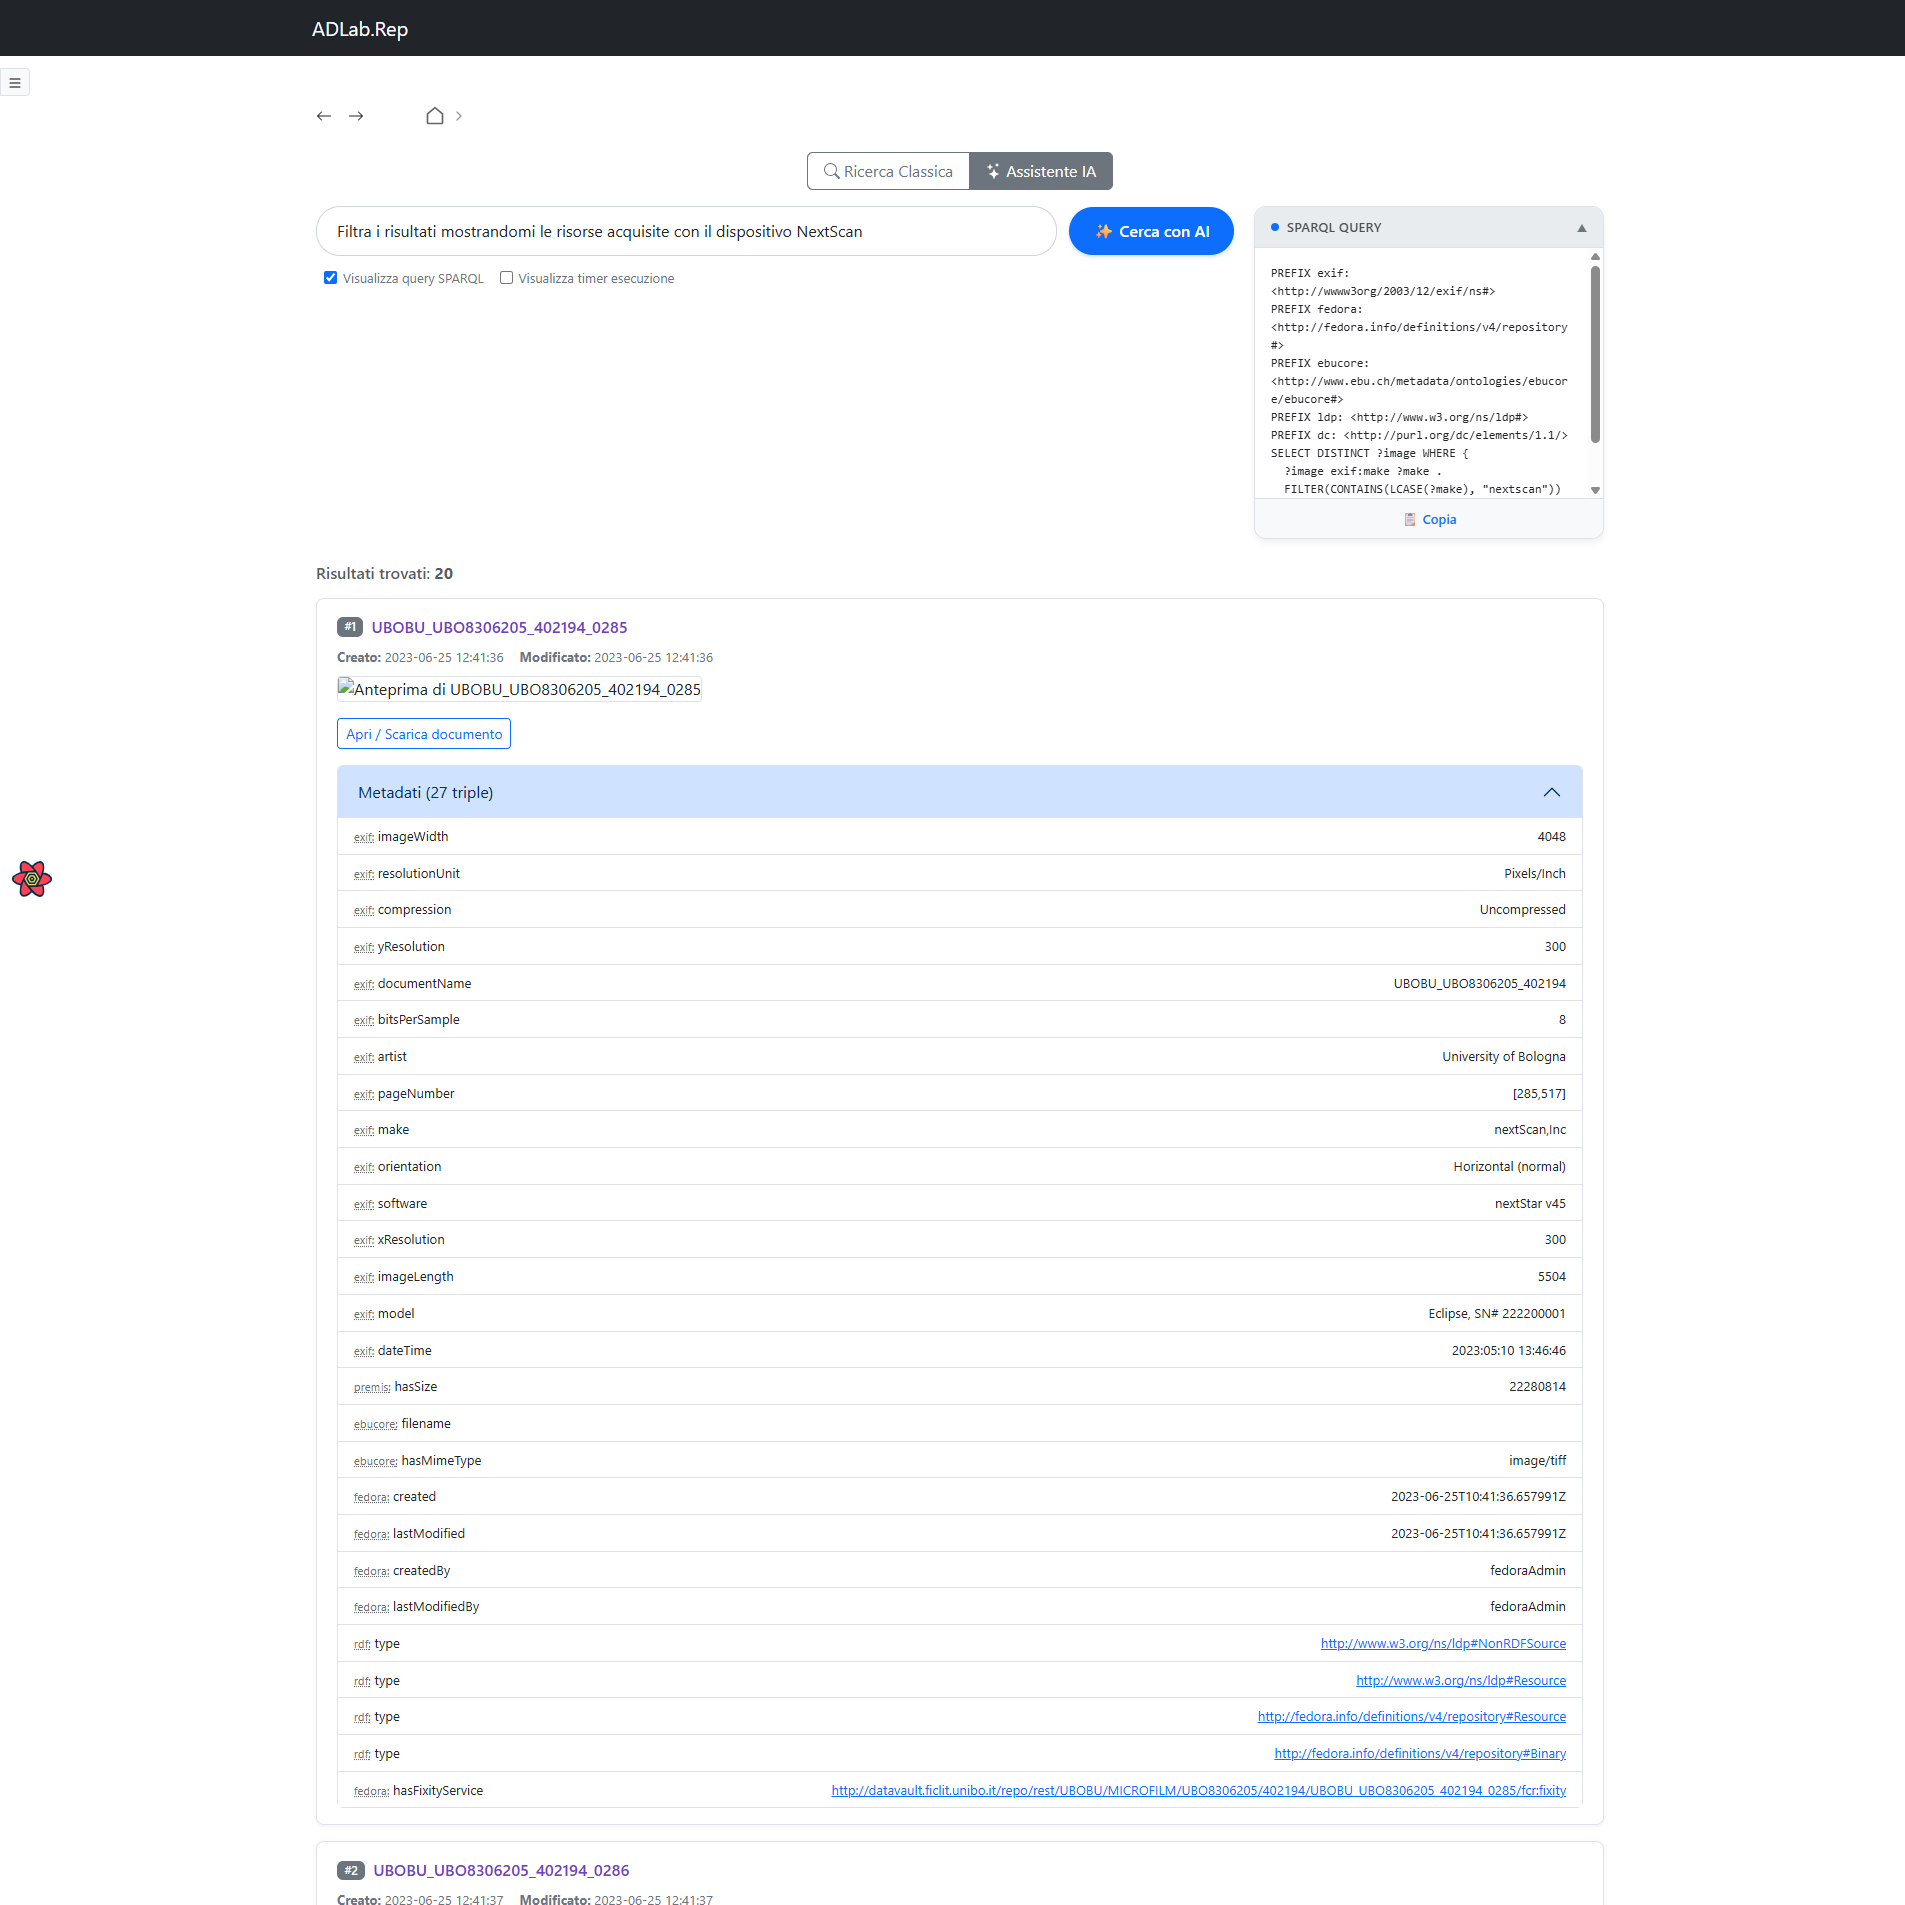
\includegraphics[width=\textwidth]{img/caso_uso_1.png} 
    \end{minipage}
    \caption{Caso d'uso 1: A sinistra la query SPARQL generata e sanitizzata, a destra l'estrazione delle risorse corrispondenti al dispositivo.}\label{fig:caso_uso1}
\end{figure}

\textbf{Risoluzione del problema}: Oltre a delegare all'LLM l'onere della traduzione del linguaggio naturale nel predicato corretto (\texttt{exif:make}), questo scenario dimostra la resilienza dell'architettura. Il modulo di sanitizzazione nel backend intercetta l'input e mantiene inalterati i prefissi (URI) per allinearli ai dati reali presenti in Blazegraph (es.\ il refuso storico \texttt{wwww3org}), mitigando eventuali discrepanze strutturali senza interrompere l'esperienza utente.

\subsection{Caso d'uso 2: disambiguazione semantica dell'autore}\label{subsec:cu2}
\textbf{Attore}: un responsabile di un progetto di digitalizzazione o ricercatore interessato alla provenienza materiale dello scatto.\\
\textbf{Input testuale}: ``Filtra le risorse mostrandomi i file in cui l'autore dello scatto è University''.

\begin{figure}[H]
    \centering
    \begin{minipage}[c]{0.48\textwidth}
\begin{lstlisting}[basicstyle=\ttfamily\scriptsize, breaklines=true]
PREFIX exif: <http://wwww3org/2003/12/exif/ns#>
# [...]

SELECT DISTINCT ?image WHERE {
  ?image exif:artist ?artist .
  FILTER(CONTAINS(LCASE(?artist), "university"))
}
LIMIT 20
\end{lstlisting}
    \end{minipage}\hfill
    \begin{minipage}[c]{0.48\textwidth}
        % INSERISCI QUI LO SCREENSHOT DEL RISULTATO DI QUESTA QUERY
        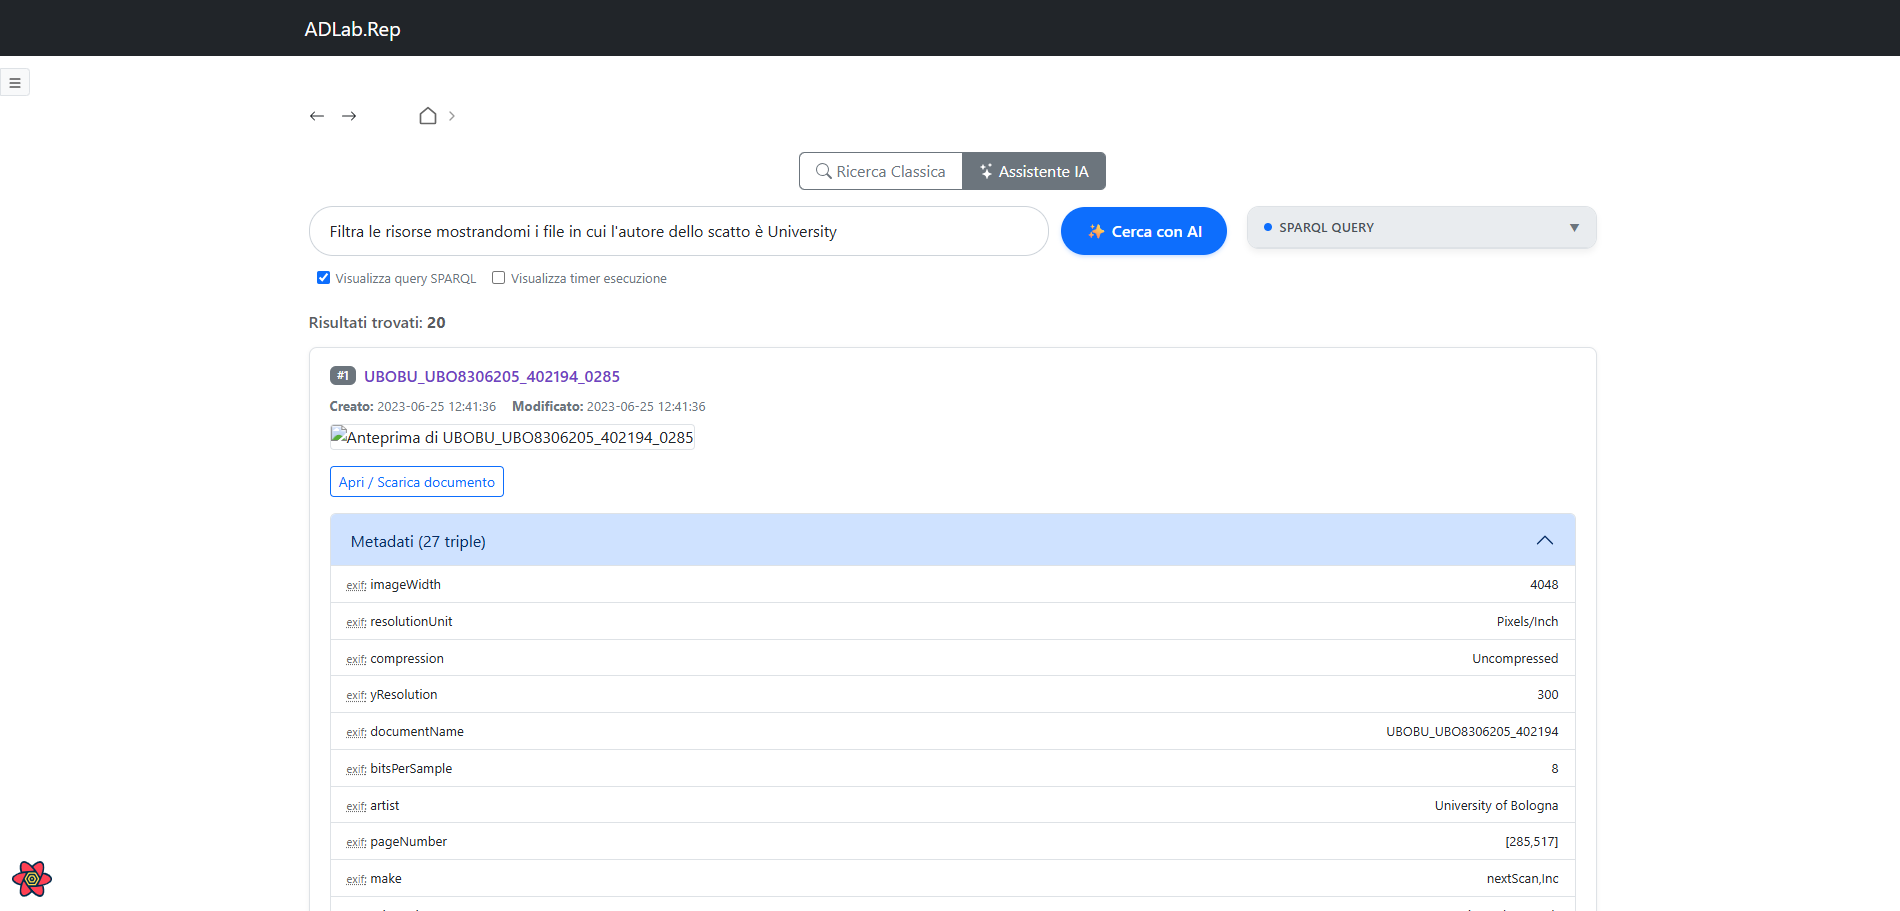
\includegraphics[width=\textwidth]{img/caso_uso_2.png} 
    \end{minipage}
    \caption{Caso d'uso 2: Disambiguazione semantica dell'autore e visualizzazione dei risultati.}\label{fig:caso_uso2}
\end{figure}

\textbf{Risoluzione del problema}: Questo scenario evidenzia la capacità dell'LLM di operare una corretta disambiguazione semantica. Il modello comprende l'intento dell'utente distinguendo l'autore materiale dello scatto (\texttt{exif:artist}) dall'utente responsabile del caricamento nel Data Vault (\texttt{fedora:createdBy}). Inoltre, l'impiego di una ricerca per match parziale aggira nativamente fenomeni di ``rumore linguistico'' che possono insorgere durante la generazione della query SPARQL.\@

\subsection{Caso d'uso 3: ricerca multi-criterio con filtro temporale}\label{subsec:cu3}
\textbf{Attore}: un ricercatore che vuole analizzare la produzione digitale filtrandola all'interno di un preciso arco temporale.\\
\textbf{Input testuale}: ``Mostrami tutte le risorse comprese tra l'anno 2023 e il 2026.\@''.

\begin{figure}[H]
    \centering
    \begin{minipage}[c]{0.48\textwidth}
\begin{lstlisting}[basicstyle=\ttfamily\scriptsize, breaklines=true]
PREFIX exif: <http://wwww3org/2003/12/exif/ns#>
# [...]

SELECT DISTINCT ?image WHERE {
  ?image exif:dateTime ?date .
  FILTER(STR(?date) >= "2023" && STR(?date) <= "2026")
}
LIMIT 20
\end{lstlisting}
    \end{minipage}\hfill
    \begin{minipage}[c]{0.48\textwidth}
        % INSERISCI QUI LO SCREENSHOT DEL RISULTATO DI QUESTA QUERY
        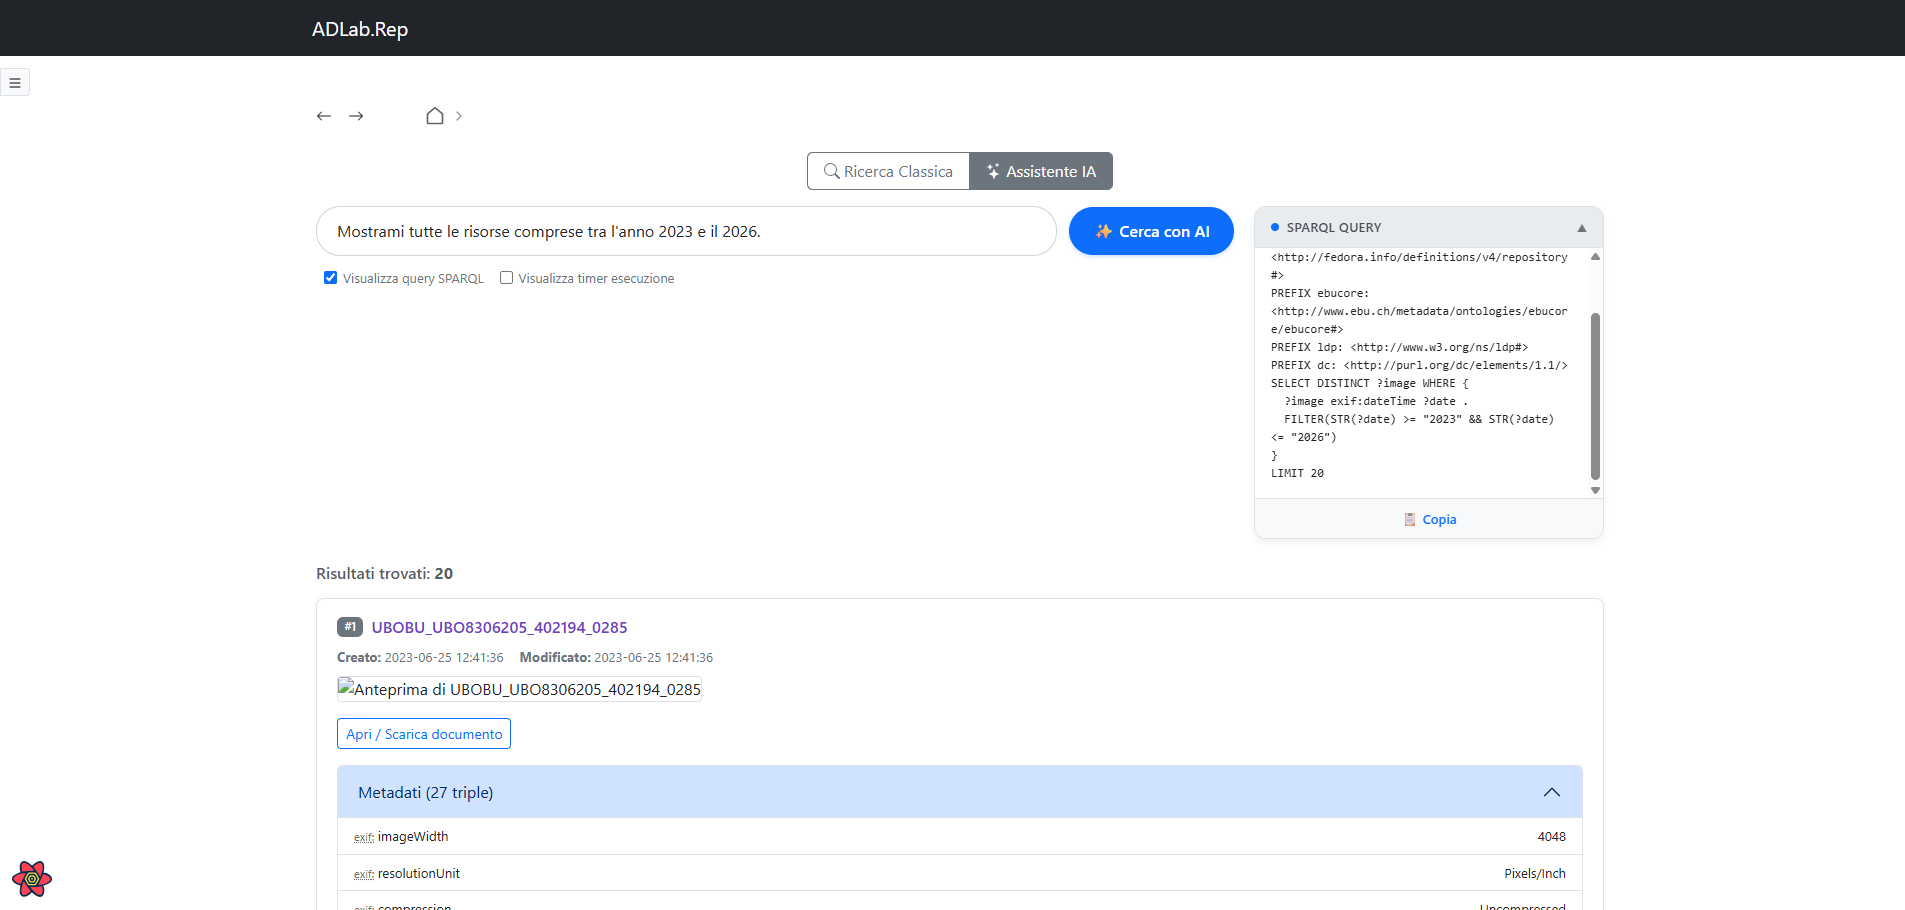
\includegraphics[width=\textwidth]{img/caso_uso_3.png} 
    \end{minipage}
    \caption{Caso d'uso 3: Applicazione logica del range temporale ed estrazione delle immagini.}\label{fig:caso_uso3}
\end{figure}

\textbf{Risoluzione del problema}: L'estrazione basata su range temporali richiede una sintassi SPARQL rigorosa e insidiosa per un utente non tecnico. Il sistema individua automaticamente il predicato \texttt{exif:dateTime} e costruisce i costrutti logici di comparazione testuale (\texttt{>=} e \texttt{<=}). Parallelamente, il backend normalizza autonomamente il formato testuale delle date per assicurare la piena compatibilità della query finale con l'ontologia prescritta dal repository istituzionale.

\section{Conclusioni del capitolo}\label{sec:conclusioni_cap3}
In questo capitolo abbiamo presentato il prototipo e la sua interfaccia, rispondendo attivamente alle criticità sollevate nel \cref{chap:contesto}:
\begin{enumerate}
    \item Il problema della \textbf{``scatola vuota''} e la paralisi decisionale (Legge di Hick) sono stati superati adottando un'interfaccia basata unicamente sull'input testuale naturale.
    \item L'obbligo di conoscere schemi complessi (es.\ prefissi EXIF o Dublin Core) è stato demandato al backend, azzerando il carico cognitivo per l'utente finale.
    \item La rigidità formale di SPARQL è stata assorbita dall'LLM, che agisce come mediatore invisibile.
\end{enumerate}

Avendo chiarito \textit{cosa} fa il sistema e \textit{come} risolve i problemi architetturali lato utente, il \cref{chap:implementazione} approfondirà il \textit{dietro le quinte} tecnologico: la struttura del backend, l'ottimizzazione del proxy Vite e il delicato processo di fine-tuning del modello linguistico.